%\documentclass[conference]{IEEEtran}
\documentclass[10pt, conference, letterpaper]{IEEEtran}
%% INFOCOM 2013 addition:
\makeatletter
\def\ps@headings{%
\def\@oddhead{\mbox{}\scriptsize\rightmark \hfil \thepage}%
\def\@evenhead{\scriptsize\thepage \hfil \leftmark\mbox{}}%
\def\@oddfoot{}%
\def\@evenfoot{}}
\makeatother
\pagestyle{headings}

\usepackage{amsmath}
\usepackage{algorithm}
\usepackage{algorithmic}
\usepackage{graphicx}
\usepackage{cite}
%\usepackage{mathrsfs}
\usepackage[bookmarks=false]{hyperref}
\usepackage{array}
\usepackage{cases}
\usepackage{booktabs}
\usepackage{multirow}
\usepackage{threeparttable}


%
%\begin{flushleft}\fontsize{8.5pt}{0.6\baselineskip}\selectfont{Remarks: 1) ``$-$" means the algorithm is not applicable to
%oblivious blind rendezvous; 2) ETTR means expected time to rendezvous (note: MMC cannot guarantee rendezvous in bounded time); 3) $P$ is the smallest prime number larger than $N$, $P=O(N)$. 4) $k_a$ and $k_b$ denote the numbers of two users' available channels; 5) SCH in this paper is only suitable for synchronous users.
%}\end{flushleft}


\newtheorem{property}{Property}[section]
\newtheorem{theorem}{Theorem}
\newtheorem{lemma}{Lemma}[section]
\newtheorem{claim}[lemma]{Claim}
\newtheorem{remark}{Remark}[section]
\newtheorem{definition}{Definition}[section]
\newtheorem{corollary}{Corollary}
\newtheorem{problem}{Problem}

\ifCLASSINFOpdf

\else

\fi

\ifCLASSOPTIONcompsoc
\usepackage[tight,normalsize,sf,SF]{subfigure}
\else
\usepackage[tight,footnotesize]{subfigure}
\fi

% correct bad hyphenation here
\hyphenation{op-tical net-works semi-conduc-tor}


\begin{document}


\bibliographystyle{plain}

\title{Improved Rendezvous Algorithms and a Semi-Synchronous Model for Heterogeneous Cognitive Radio Networks}

%\author{\IEEEauthorblockN{
%Zhaoquan Gu\IEEEauthorrefmark{1}, Haosen Pu\IEEEauthorrefmark{1}, Qiang-Sheng Hua\IEEEauthorrefmark{2}, and
%Francis C.M. Lau\IEEEauthorrefmark{3}}
%
%\IEEEauthorblockA{\IEEEauthorrefmark{1}Institute for Interdisciplinary Information Sciences, Tsinghua University,
%Beijing, China\\}
%\IEEEauthorblockA{\IEEEauthorrefmark{2}School of Computer Science $\&$ Technology, Huazhong University of Science and Technology, China\\}
%\IEEEauthorblockA{\IEEEauthorrefmark{3}Department of Computer Science, The University of Hong Kong, Hong Kong, China\\}
%}

\maketitle


\begin{abstract}
Cognitive Radio Network (CRN) is a promising technique aiming at solving the wireless spectrum scarcity problem. Rendezvous is the fundamental process of CRN. Heterogeneous CRN allows different users to have different sensing abilities. We are devoted to design faster rendezvous algorithms for heterogeneous CRN. First, we design a non-anonymous rendezvous algorithm which uses users' IDs. This algorithm can guarantee rendezvous for any two users $i,j$ in $(l+1)(|V_i|+2)(|V_j|+2)$ timeslots, where $l$ is the length of ID and $|V_i|,|V_j|$ are the size of the set of available channels for user $i$ and $j$ respectively. Second, we study the two-radio rendezvous problem where every user is equipped with two CRNs and propose a rendezvous algorithm for two-radio problem without using users' IDs. This algorithm can guarantee rendezvous for any two users $i$ and $j$ in $min\{|V_i||V_j|\}max\{P_i,P_j\}$ timeslots, where $P_i$ and $P_j$ are the smallest primes which are not less than $|V_i|$ and $|V_j|$ respectively. Third, we propose a semi-synchronous model which suppose there exists a global clock but users don't need to start rendezvous process simultaneously. We also design a rendezvous algorithm for semi-synchronous model which can guarantee rendezvous for any two users in $N$ timeslots, where $N$ is the overall amount of channels in the network. We show that our rendezvous algorithms have full rendezvous degrees. All of our algorithms can be used in multi-user scenario. We conduct plenty of experiments comparing our algorithms with state-of-the-art rendezvous in different scenarios, which corroborate our analysis.
\end{abstract}


\begin{IEEEkeywords}
Heterogenous Cognitive Radio Network, Rendezvous Algorithms, Non-Anonymous, Two-Radio, Semi-Synchronous Model
\end{IEEEkeywords}

\section{Introduction}
The wireless spectrum is very important for the transmission of wireless signals. However, the wireless spectrum scarcity problem is becoming more and more severe due to the rapid growth of wireless devices. Cognitive Radio Network (CRN) is a solution for this problem. In CRN, the users are divided into primary users (PUs) and secondary users (SUs) . A PU owns one or more licensed spectrums while a SU needs to search for ``empty" licensed spectrums which are not being occupied by PUs \footnote{Unless specifically pointed out, ``users" in the rest of this paper refer to SUs.}.

CRN involves many important problems including broadcasting, routing, data gathering and neighbor discovery. \emph{Rendezvous} is the fundamental task of CRN, which targets finding a common frequency band (channel) for different users to communicate on. Before rendezvous completes, a user may even not aware of the existence of another user, let alone exchange information.

To solve rendezvous problem, many solutions have been proposed. Some works requires a central controller or a common control channel (CCC) to achieve rendezvous. However, when the number of users exceeds the capacity of the central controller or CCC, this method will become invalid. And it is not safe from the perspective of information security, for the probability of adversary attacks. Hence, some researchers proposed some algorithms without central controller or CCC, which are called blind rendezvous algorithms. Blind rendezvous algorithms are more practical than CCC based rendezvous algorithms.

Channel Hopping (CH) technique is widely used in blind rendezvous algorithms. In CH algorithms, users hop to channels according to predefined sequences. Time is divided into timeslots with equal length, which is enough for two users to establish a communication link when they are on a channel at the same time. The length of a timeslot can be set to be 10 ms under IEEE 802.22, which is a recommended standard for CRN.

\begin{table*}[!t]
\renewcommand{\arraystretch}{1.3}
 \caption{\upshape Comparisons between rendezvous algorithms }
\centering
\begin{tabular}{|c|c|c|c|c|c|c|}
\hline
Algorithm & MTTR & RD & Synchronous & Non-Anonymous &Non-Oblivious & Two-Radio\\
\hline
JS & 3NP(P-G) +3P & 100\% & $ \times$ & $ \times $ & $ \surd$ & $\times$\\
\hline
DRDS & $3P^2 + 2P$ & 100\% &$\times$ &$\times$ &$\surd$ & $\times$\\
\hline
CBH & $2l_pP^2$ & 100\% & $\times$ & $\surd$ & $\times$ & $\times$\\
\hline
HH & $3|C_a||C_b|$ &$ <100\%$ &$\times$ &$\times$& $\surd $ &$\times$\\
\hline
advanced HCH & $(log M + loglog M)P_iP_j$ & 100\% & $\times$ &$\surd$ &$\times$ &$\times$\\
\hline
MTP & $O((max\{|V_i|,|V_j|\})^2loglog N$ & 100\%& $\times$ & $\times$ & $\times$ &$\times$\\
\hline
NAH(this paper) & $log M (P_i + 2)(P_j +2)$ & 100\% &$\times $ & $\surd$ & $\times$ & $\times$\\
\hline
TRAH(this paper) & $min\{|V_i||V_j|\}max\{P_i,P_j\}$ &100\% &$\times $ & $\times$ & $\times$ &$\surd$\\
\hline
SSH(this paper) & $N$ & 100\% & semi-synchronous &$\times$ &$\times $ & $\times$ \\
\hline
\end{tabular}
\end{table*}


Rendezvous algorithms can be judged according to some common metrics, such as \emph{Expected Time To Rendezvous (ETTR)}, \emph{Maximum Time To Rendezvous (MTTR)}, \emph{Rendezvous Degree (RD)}. \emph{Time To Rendezvous (TTR)} is the number of timeslots consumed to achieve rendezvous, which begins counting as soon as the latest user begins hopping. ETTR is the average TTR of an algorithm. MTTR is the maximum TTR needed to achieve rendezvous. In other words, MTTR is the TTR in the worst case. It is obvious that two users can have more than one common channel, RD is the ratio of the number of distinct rendezvous channels of an algorithm to the total number of common channels. It is obvious that the larger RD is, the more channels two users can rendezvous on. Because a channel can be occupied by a PU and not useful for rendezvous, the larger RD is, the better.

In this paper, we introduce some simple but efficient rendezvous algorithms under different scenarios. The following are the main contributions of our paper:
\begin{itemize}
\item[1)] We propose a non-anonymous heterogeneous rendezvous algorithm which outperforms state-of-the-art non-anonymous heterogeneous rendezvous algorithms.
\item[2)] We propose a two-radio heterogeneous rendezvous algorithm which outperforms the state-of-the-art two-radio heterogeneous rendezvous algorithm.
\item[3)] We formulate the concept of semi-synchronous model and propose a semi-synchronous rendezvous algorithm which is a feasible and has a MTTR of $N$, which is least in all the existing rendezvous algorithms.
\item[4)] We conduct lots of experiments to compare our algorithms with state-of-the-art algorithms.
\end{itemize}


The rest of this paper is organized as follows. Section \uppercase\expandafter{\romannumeral2} introduces the background and some related works. Section \uppercase\expandafter{\romannumeral3} introduces different categories of models for rendezvous problem and problem formulation. Section \uppercase\expandafter{\romannumeral4} presents a non-anonymous heterogeneous rendezvous algorithm and analyzes its performance. Section \uppercase\expandafter{\romannumeral5} presents a two-radio heterogeneous rendezvous algorithm and analyzes its performance. Section \uppercase\expandafter{\romannumeral6} presents a semi-synchronous heterogeneous rendezvous algorithm and analyzes its performance. Simulation results are displayed in Section Section \uppercase\expandafter{\romannumeral7}. And we conclude this paper in Section \uppercase\expandafter{\romannumeral8}.




\section{Background and Related Works}


\subsection{Prime number and Co-prime Numbers}
Prime number is a very important concept in number theory. We first introduce the definition of prime number:
\begin{definition}
A prime number is a natural number which is larger than 1 and can be divided with no remainder only by 1 and itself.
\end{definition}

The smallest prime number is 2. There is an important theory about prime number:
\begin{theorem}
If n is a positive integer and $n \ge 2$, there must exists at least one prime number between n and 2n.
\end{theorem}

Then we introduce the definition of composite number:
\begin{definition}
A composite number is a natural number which is larger than 1 and has factors besides 1 and itself.
\end{definition}

The smallest composite number is 4. There is a property about prime and composite numbers:

\begin{lemma}
Any positive integer larger than 1 is either a prime number or a composite number.
\end{lemma}

Then we introduce the definition of co-prime numbers:
\begin{definition}
Two nonzero natural integers a and b are said to be co-prime if the only common factor which could divide them with no remainder is 1.
\end{definition}

Co-prime numbers have many important properties:
\begin{lemma}
If a and b are co-prime, the least common multiple of them is their product: $a \times b$.
\end{lemma}
\begin{lemma}
If a and b are two consecutive positive integers, a and b are co-prime.
\end{lemma}
\begin{lemma}
If a and b are two consecutive positive odd numbers, a and b are co-prime.
\end{lemma}
\begin{lemma}
Suppose a is a prime number and b is a composite number. If a is larger than b, they are co-prime. If b is larger than a, but b is not a multiple of a, they are co-prime.
\end{lemma}

We then introduce an important theorem for rendezvous:
\begin{theorem}
\label{theo}
If m and n are co-prime numbers, then for any integer a, the integers $a, a + n, a + 2n,\cdots, a+(m-1)n$ are m distinct numbers under modulo-p arithmetic.
\end{theorem}
\begin{IEEEproof}
Choose any two integers from $a, a+n, a + 2n,\cdots, a+(m-1)n$, the absolute value of their difference is kn, where $0 < k < m$. If kn mod m equal 0, then $kn = lm$, where l is a positive integer. Then kn or lm is a common multiple of m and n. From Lemma 2.2 we know mn is the least common multiple of m and n, and because $0 < k < m$, kn is a common multiple of m and n that is less than mn, which is a contradiction. Hence, Theorem \ref{theo} holds.
\end{IEEEproof}

\begin{figure}[!t]
\centering
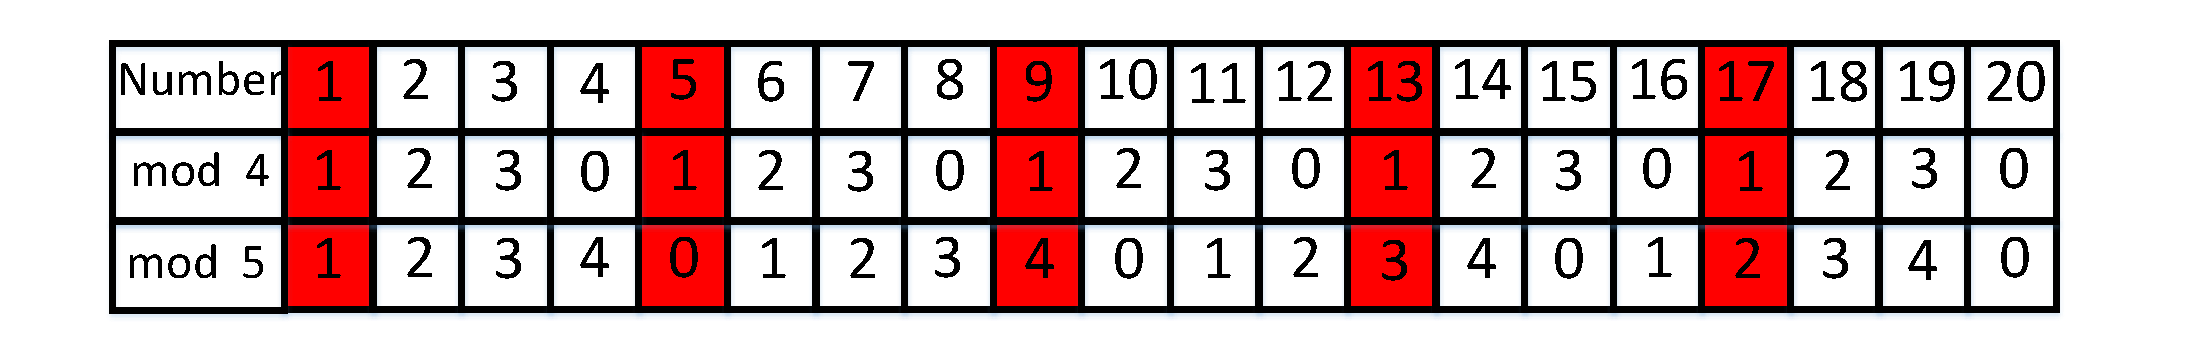
\includegraphics[width=1\columnwidth]{theo}
\caption{An example of Theorem \ref{theo}.}
\label{exp1}
\end{figure}

Fig. \ref{exp1} illustrates an example of Theorem \ref{theo}. In Fig. \ref{exp1}, the first row is a string of numbers starting from 1. The second row is the results of these numbers under modulo 4 arithmetic. The third row is the results of these numbers under modulo 5 arithmetic. We can clearly see that 1, 5, 9, 13, 17 all correspond to 1 under modulo 4 arithmetic, but correspond to 1, 0, 4, 3, 2 respectively under modulo 5 arithmetic, which are all the possible results under modulo 5 arithmetic. Theorem \ref{theo} plays an important role in rendezvous algorithms and is the main tool we use to design the following algorithms.
\subsection{Related Works}

\section{Models and Problem Formulations}
In this section, we will introduce the foundation model and some other models which are based on the foundation model. Models are of great importance in the design of rendezvous algorithms, because models constrain the resources that we can use. Hence, we need to design different algorithms under different models to achieve high performance for rendezvous process. We will also give the formulation for rendezvous problem in this section.
\subsection{Foundation Model}
Suppose there are M users in the network. Suppose the licensed spectrum is divided into n channels which are non-overlapping. Denote the set of channels as $U=\{1,2,\cdots,n\}$, where n is the total number of channels in U. We assume that every user in the network is equipped with a CRN. User i can sense a set of channels as
$C_i=\{c_{i1},c_{i2},\cdots,c_{in_i} \}$, where $n_i$ is the number of channels in set $C_i$. A channel is available to user i when it is not occupied by a PU and it is in $C_i$. User i has a set of available channels as $V_i = \{v_{i1},v_{i2},\cdots,v_{im_i}\}$, where $m_i$ is the number of channels in set $V_i$. For simplicity, we suppose that $V_i$ doesn't change during the rendezvous process. Let the length of every timeslot be 2t, where $t=10ms$ according to IEEE 802.22.

\begin{figure}
\centering
\subfigure[case 1]{
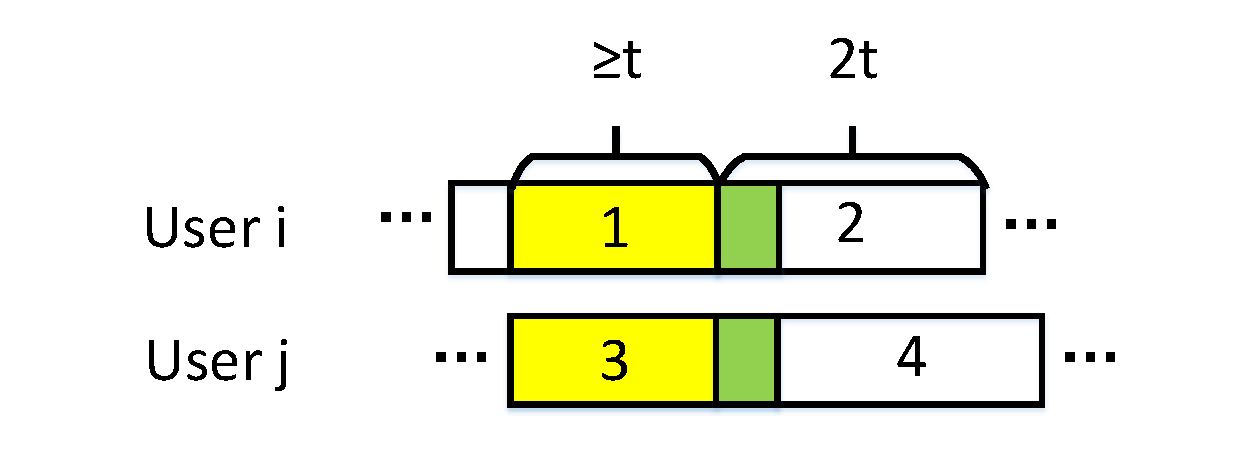
\includegraphics[width=1.6in]{olp1}
\label{olp1}
}
\subfigure[case 2]{
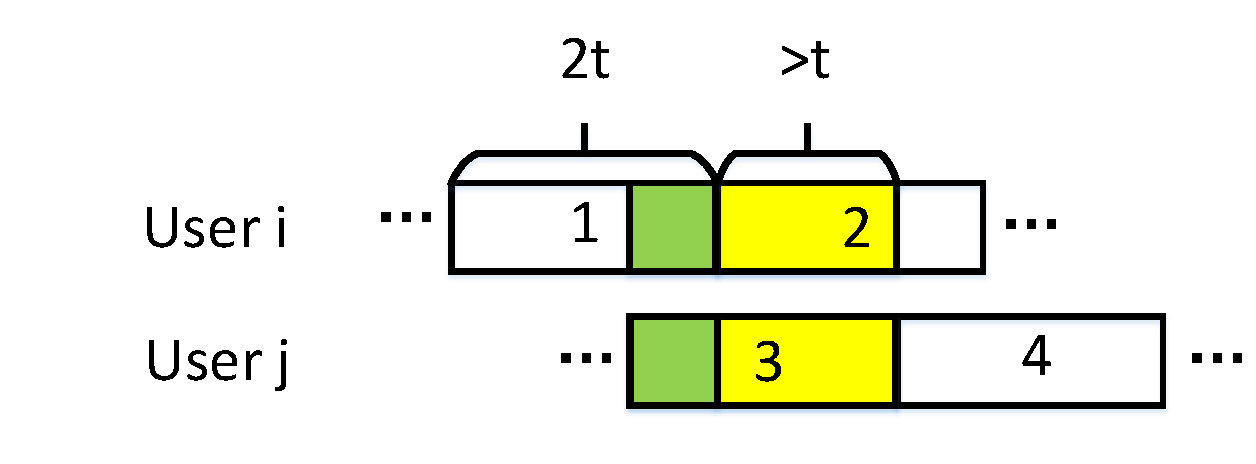
\includegraphics[width=1.6in]{olp2}
\label{olp2}
}
\caption{An example of different cases of timeslot overlapping.}
\label{overlap}
\end{figure}

Because the lengths of all users' timeslots are equal, user j's one timeslot can overlap with at most two consecutive timeslots of user i. Fig. \ref{overlap} illustrates this problem in two cases. Suppose timeslot 3 is one timeslot of user j. And the left timeslot of user i which overlaps with timeslot 3 is timeslot 1. The right timeslot of user i which overlaps with timeslot 3 is timeslot 4. The yellow part stands for the overlapping part of timeslot 1 and 3, while the green part stands for the overlapping part of timeslot 2 and 3. In Fig. \ref{olp1}, the length of the yellow part is greater than or equal to t. In Fig. \ref{olp2}, the length of the green part is greater than t.
There is a special case that the length of the yellow part or the green part is zero, which means that the timeslots of user i and user j are aligned.
Hence, no matter when the users start their rendezvous process, the maximum overlap of their timeslots is at least t, which is enough for two users to find each other and exchange information.Foundation model is the basis of other models we will introduce in the following subsections.

\subsection{Oblivious and Non-Oblivious Models}
The difference between oblivious and non-oblivious models is whether there exists a global label for every channel in $U$ and users label channels as same as their global labels. In oblivious model, there doesn't exist any global label and every user labels channels in its own way. For example, for the same channel, denote it as c, user i can label it as 1 while user j can label it as 2. In non-oblivious model, there exist global labels for channels such as $U=\{1,2,\cdots,n\}$ where we label the i-th channel in U as i. And the label of every channel for every user is as same as its global label.  It is obvious that designing rendezvous algorithms for oblivious model is at least not easier than non-oblivious model, since in non-oblivious model, we could use the labels of channels as an extra resource for designing rendezvous algorithms.

\subsection{Anonymous and Non-Anonymous Models}
The difference between an is whether each user in the network has a unique ID. In anonymous model, there doesn't exist a unique ID for each user. Hence, a user can't be distinguished from the other users. In non-anonymous model, there exists a unique ID for each user. Hence, a user is easily distinguishable from the other users. Designing rendezvous algorithms for non-anonymous model is easier than anonymous model, because we can use IDs, which will be shown very powerful for rendezvous process.

\subsection{Synchronous, Asynchronous and Semi-Synchronous Models}
In the previous works, there exist synchronous and asynchronous rendezvous algorithms. In synchronous model, there exists a global clock, and time is divided into equal timeslots. And every user start their rendezvous process from the same timeslot. In asynchronous model, there doesn't exist any global clock, time is divided into equal timeslots according to their local clock. And every user can start its own rendezvous process at any time.

In this paper, we introduce a new model about timing, which is semi-synchronous model. In semi-synchronous model, there exists a global clock, and time is divided into equal timeslots. However, every user can start its own rendezvous process at any timeslot. Though synchronous model is difficult to implement, semi-synchronous model is practical. There exist many techniques to achieve time giving, such as GPS timing, Beidou satellite time giving, CSAO time giving and so on. These time services have high precision. For example, GPS timing can achieve 10 nanosecond level precision. Because our timeslot is 20 ms long, this level of precision is enough for our use.

We need to point out that different models in different subsections can be combined to generate a new model. We will propose some algorithms for three combined models.

\subsection{Problem Formulations}
In this paper, we focus on designing rendezvous algorithms for two-user scenario, because it is the fundamental process for multiple-user rendezvous. Two-user rendezvous algorithms can be expanded into multiple-user rendezvous algorithms. Then we give the formulations of the three problems we will solve:

\begin{problem}
Design a rendezvous algorithm which has low MTTR and highest RD for heterogeneous non-anonymous model.
\end{problem}

\begin{problem}
Design a two-radio rendezvous algorithm which has low MTTR and highest RD for heterogeneous anonymous  model.
\end{problem}


\begin{problem}
Design a rendezvous algorithm which has low MTTR and highest RD for semi-heterogeneous model.
\end{problem}

\section{Non-Anonymous Heterogeneous Rendezvous Algorithm}
In this section, we will propose a heterogeneous non-anonymous rendezvous algorithm.
The main idea of this algorithm is to create a channel hopping sequence composed of $\left \lceil log_2 M \right \rceil + 1$ subsequences. We first propose an algorithm to generate the subsequences to be used.

\begin{algorithm}
\caption{Subsequence Generating Algorithm}
\label{alg2}
\begin{algorithmic}[1]
\STATE Input: the set of available channels $V=\{v_1,v_2,\cdots,v_m\}$, and length $L$;
\STATE Initialize $i :=0$;
\WHILE {$i < L$}
\IF{$i \le m$}
\STATE $S[i] := v_i$;
\ELSE
\STATE Randomly choose a channel from $V$, denote it as $c$;
\STATE $S[i] := c$;
\ENDIF
\STATE $i:=i+1;$
\ENDWHILE
\STATE Output: Sequence $S$.
\end{algorithmic}
\end{algorithm}

The main idea of Alg.\ref{alg2} is to generate a subsequence $S$ with length $T$ according to $V$. The process is rather simple. We fill the first $m$ elements in $S$ with the channels in $V$. For the last $(T-m)$ elements, we randomly pick channels from $V$ to fill them. Fig.{\ref{exp-seq}} shows an example of Alg.\ref{alg2}, in which $V=\{v_1,v_2,\cdots,v_8\}$ and $T=10$. We can clearly see that the first 8 elements are set to be $v_1,v_2,\cdots,v_8$ respectively. The last $10-8=2$ elements are colored in green, which means that they are randomly picked from $V$.

\begin{figure}[!t]
\centering
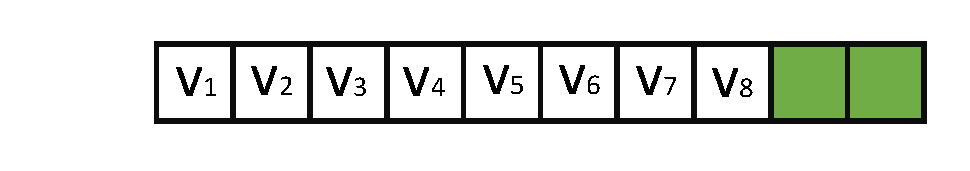
\includegraphics[width=1\columnwidth]{seq}
\caption{An example of Alg. {\ref{alg2}}.}
\label{exp-seq}
\end{figure}


\begin{algorithm}
\caption{Non-Anonymous Heterogeneous Rendezvous Algorithm}
\label{alg3}
\begin{algorithmic}[1]
\STATE Input: the set of available channels $V=\{v_1,v_2,\cdots,v_m\}$, and its ID whose length is $\left \lceil log_2 M  \right \rceil$ bits;
\STATE Find the smallest prime $P$ that ensure $P \ge m$;
\IF{P==3}
\STATE $P:= 5$;
\ENDIF
\STATE Initialize $t := 0$;
\STATE Invoke Alg.\ref{alg2} to generate three sequences $S_1,S_2,S_3$ with channel set V and length P, P+1, P+2 respectively;
\WHILE{Not rendezvous}
\IF{$ t\;\% \;(\left \lceil log_2M \right \rceil  +1) \neq 0$}

  \IF{ID$[t \;\% \;(\left \lceil log_2M \right \rceil  +1)]== 0$}
   \STATE Access channel

    $S_2[(t\;/\;(\left \lceil log_2M \right \rceil+1))\;mod\;(P+1)]$;
    \ELSE
    \STATE Access channel

    $S_3[(t\;/\;(\left \lceil log_2M \right \rceil+1))\;mod\; (P+2)]$;
    \ENDIF
\ELSE
\STATE Access channel

$S_1[(t\;/\;(\left \lceil log_2M \right \rceil+1))\;mod\; P]$;
\ENDIF
\STATE t := t + 1;
\ENDWHILE

\end{algorithmic}
\end{algorithm}

\begin{figure}[!t]
\centering
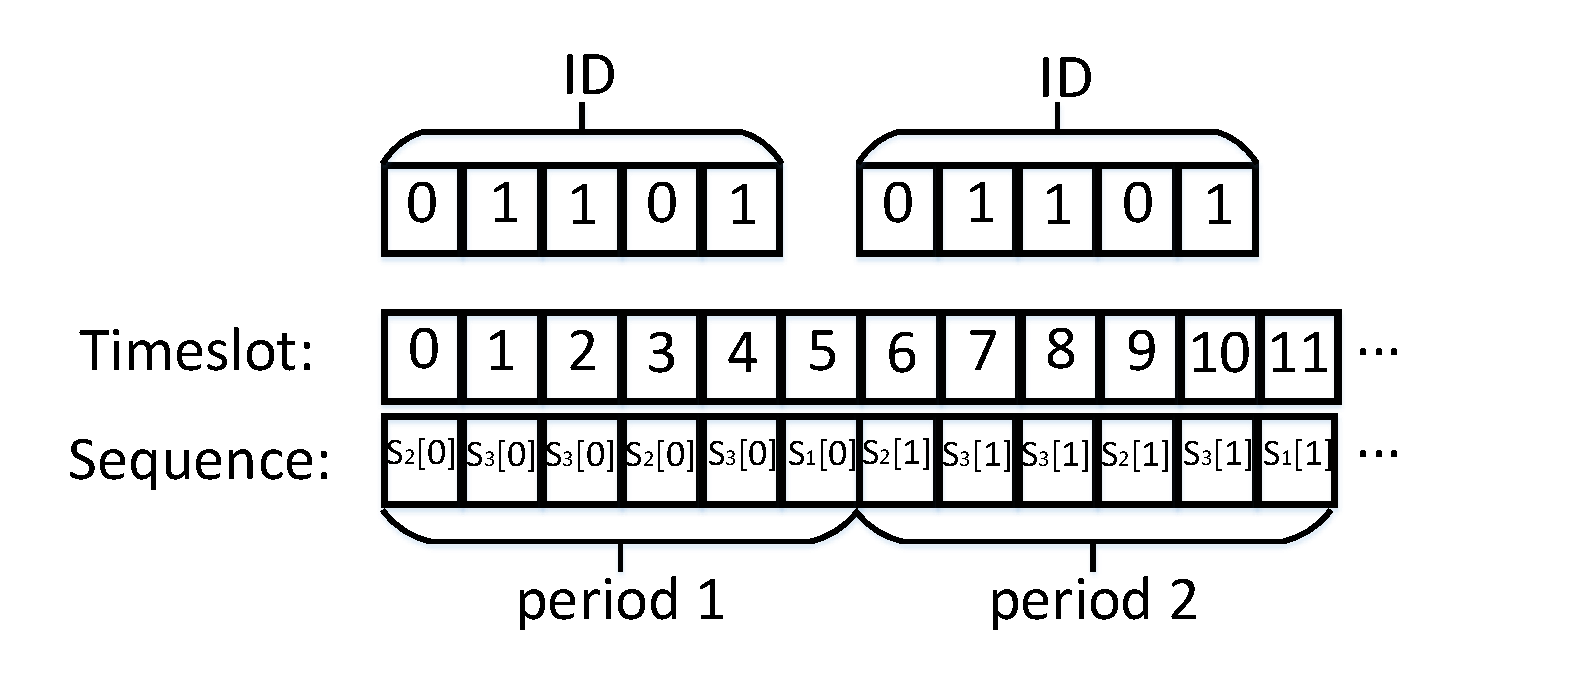
\includegraphics[width=1\columnwidth]{round}
\caption{An example of Alg. {\ref{alg3}}.}
\label{exp-alg3}
\end{figure}

In Alg.\ref{alg3}, we creates a channel hopping sequence consisting of $(\left \lceil log_2M \right \rceil +1)$ subsequences. The $(\left \lceil log_2M \right \rceil +1)$ subsequences are generated by Alg.\ref{alg2}. There are three kinds of subsequences, which are $S_1, S_2$ and $S_3$. The lengths of $S_1, S_2$ and $S_3$ are P, P+1, P+2 respectively.

Fig.\ref{exp-alg3} illustrates an example of Alg.\ref{alg3}. In this example, the length of ID is 5 and user i's ID is 01101. In round 1, the first $ \left \lceil log_2M \right \rceil$ elements of round 1 are either $S_2[0]$ or $S_3[0]$. If the corresponding digit of the i-th element in ID is 0, then the i-th element will be $S_2[0]$. If the corresponding digit of the i-th element in ID is 1, then the i-th element will be $S_3[1]$. The last element of round 1 is $S_1[0]$.

\begin{theorem}
Alg.\ref{alg3} can guarantee rendezvous for two asynchronous users in $(\left \lceil log_2M \right \rceil + 1)(P_i + 2)(P_j + 2)$ timeslots if $V_i \cap V_j \ne \emptyset$.
\end{theorem}



\begin{figure}
\centering
\subfigure[subcase 1]{
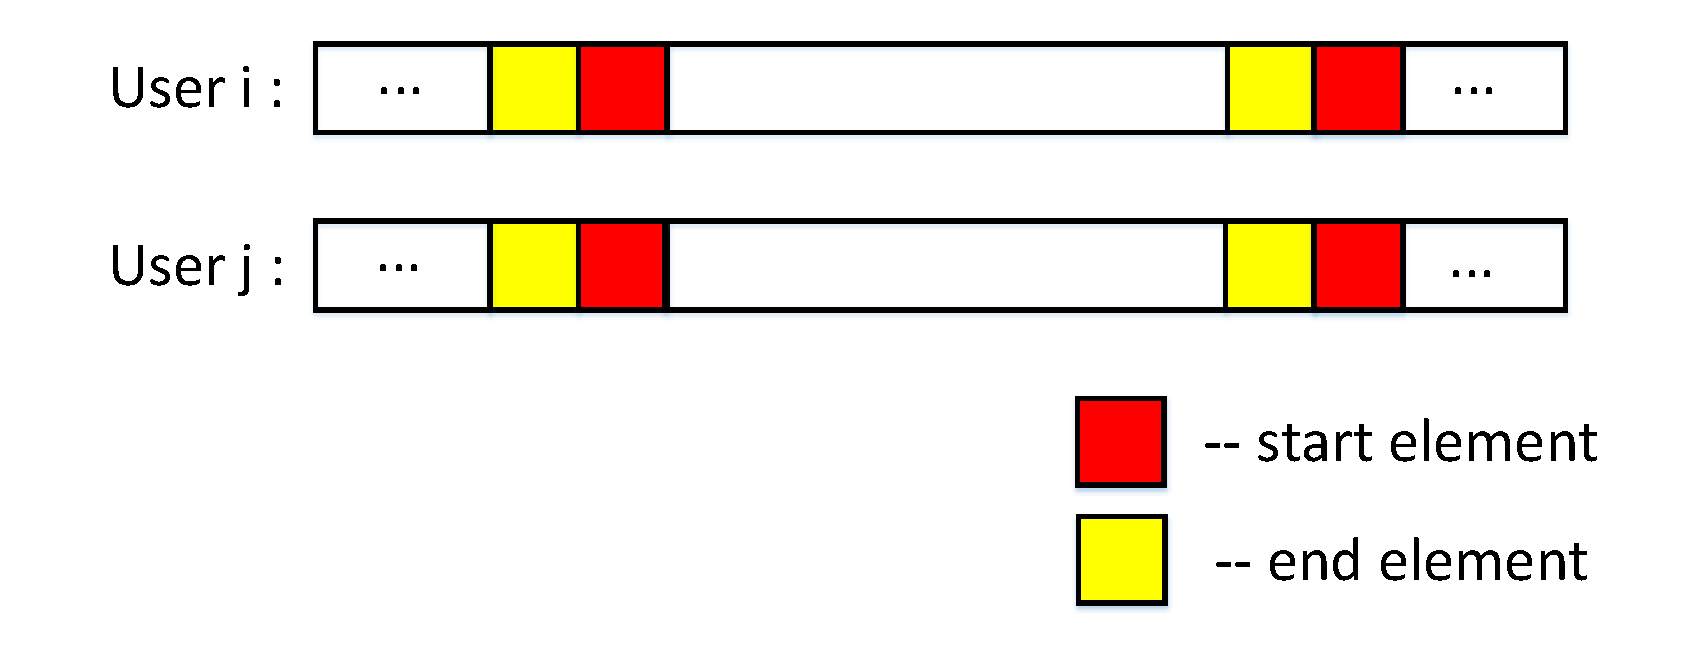
\includegraphics[width=1.6in]{case1}
\label{cs1}
}
\subfigure[subcase 2]{
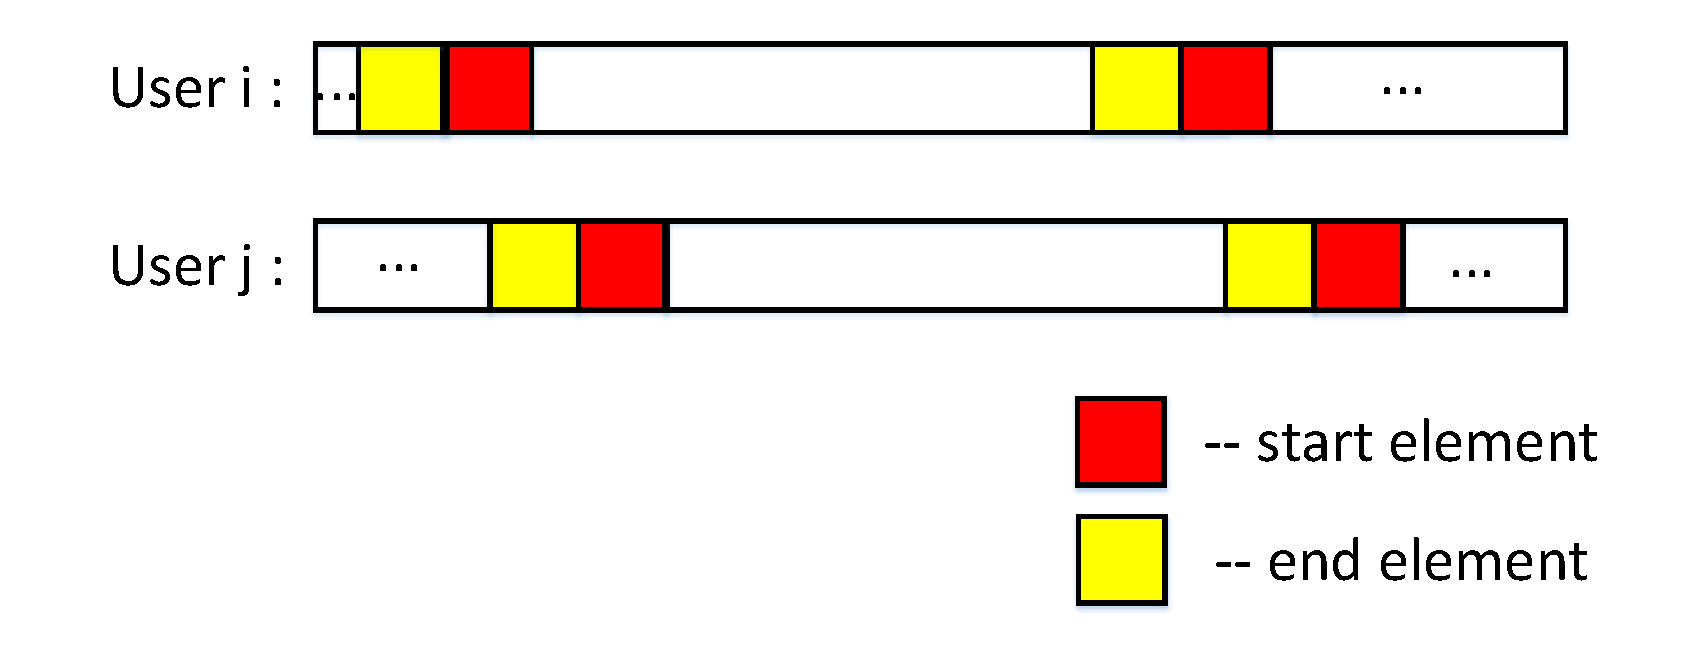
\includegraphics[width=1.6in]{case2}
\label{cs2}
}
\caption{Two subcases of case 1 and case 2.}
\label{case}
\end{figure}



\begin{IEEEproof}
We discuss in two cases:

\bfseries Case 1 \mdseries:

 Suppose $P_i = P_j$. Let $P = P_i =P_j$ We divide this case into two subcases:

\bfseries Subcase 1.1 \mdseries: Suppose user i and j's periods are aligned, as illustrated in Fig.\ref{cs1}. Because user i and user j are two different users, their ID must be different in at least one digit. Without lose of generality, suppose the k-th digit in $ID_i$ is 0 while the k-th digit in $ID_j$ is 1. Then the k-th element in user i's period corresponds to subsequence $S_{2i}$, whose length is $P+1$. The k-th element in user j's period corresponds to subsequence $S_{3j}$, whose length is $P+2$. Then in every period, one element of $S_{2i}$ will meet one element of $S_{2j}$. According to Lemma 2.3, P+1 and P+2 are co-prime. Then rendezvous can be achieved in $(\left \lceil log_2M \right \rceil + 1)(P+1)(P+2)$ timeslots according to Theorem 2, as long as user i and j have at least one common channel.

\bfseries Subcase 1.2 \mdseries: Suppose user i and j's periods are not aligned, as illustrated in Fig.\ref{cs2}. In this case, the last element in user i's period will meet one of the first $(\left \lceil log_2M \right \rceil + 1)$ elements of user j's period. The last element in user i's period corresponds to subsequence $S_{1i}$. The corresponding element of user j corresponds to subsequence $S_{2j}$ or $S_{3j}$. From Lemma 2.3 and 2.4, we know that P and P+1 are co-prome, P and P +2 are also co-prime. Hence, according to Theorem 2, rendezvous can be achieved in $(\left \lceil log_2M \right \rceil + 1)P(P+1)$ or $(\left \lceil log_2M \right \rceil + 1)P(P+2)$ timeslots respectively.

\bfseries Case 2 \mdseries: Suppose $P_i \ne P_j$.  We divide this case into two subcases:

\bfseries Subcase 2.1 \mdseries: Suppose user i and j's periods are aligned, as illustrated in Fig.\ref{cs1}. In this case, the last
element in user i's period will meet the last element in user j's period. The last element in user i's period corresponds to subsequence $S_{i1}$. The last element in user j's period corresponds to subsequence $S_{j1}$. Because $P_i \ne P_j$, rendezvous can be achieved in $(\left \lceil log_2M \right \rceil + 1)P_iP_j$ timeslots according to Theorem 2, as long as user i and j have at least one common channel.

\bfseries Subcase 2.2 \mdseries: Suppose user i and j's periods are not aligned, as illustrated in Fig.\ref{cs2}. Without lose of generality, suppose $P_i > P_j$. In this case, the last element in user i's period will meet one of the first $(\left \lceil log_2M \right \rceil + 1)$ elements of user j's period. The last element in user j's period will meet one of the first $(\left \lceil log_2M \right \rceil + 1)$ elements of user i's period. The last element in user j's period corresponds to subsequence $S_{1j}$, whose length is $P_j$. The corresponding element of user j corresponds to subsequence $S_{2i}$ or $S_{3i}$, whose lengths are $P_i +1$ and $P_i +2$ respectively. Because $P_i$ and $P_j$ are two different primes, $P_i > P_j +2$ or $P_i = P_j +2$. If $P_i > P_j + 2$, from Lemma 2.5, we know $P_i$ and $P_j + 1$ are co-prime, $P_i$ and $P_j +2 $ are co-prime. According to Theorem 2, rendezvous can be achieved in $(\left \lceil log_2M \right \rceil + 1)P_i(P_j+1)$ or $(\left \lceil log_2M \right \rceil + 1)P_i(P_j+2)$ timeslots respectively. If $P_i = P_j + 2$, then $P_i + 1 = P_2 + 3$, $P_i + 2 = P_j + 4$. If $P_j = 2$, $P_i = 2 + 2=4$ is not a prime. In Alg.\ref{alg3}, we set P to be 5 if $P=3$. Because $P_2 \ne 2$ and $P_2 \ne 3$, $P_2 + 3$ and $P_2 + 4$ can not be divided by $P_2$ without remainder. From Lemma 2.5, we know that both $P_i + 1$ and $P_i +2$ are co-prime with $P_j$. According to Theorem 2, rendezvous can be achieved in $(\left \lceil log_2M \right \rceil + 1)(P_i + 1)P_j$ or $(\left \lceil log_2M \right \rceil + 1)(P_i+2)P_j$ timeslots respectively.

Combine the above together, Theorem 3 holds.

\end{IEEEproof}

\begin{theorem}
The RD of Alg.\ref{alg3} is 100\%.
\end{theorem}

\begin{IEEEproof}
For any user, the corresponding subsequence $S_1,S_2,S_3$ all contains all the channels in its available channel set. From the proof of Theorem 3, we know that one subsequence of user $i$ will meet one subsequence of user $j$ and the lengths of the subsequences are co-prime. Denote the two subsequences as $S_i$ and $S_j$. From Theorem \ref{theo}, we know that every element in $S_i$ will meet all of the elements in $S_j$ and vice versa. Hence, the RD of Alg.\ref{alg3} is 100\%.
\end{IEEEproof}

This algorithm can also be used when the setting is oblivious. Our algorithm is more simple than the sate-of-the-art algorithm and has a less MTTR than it, which is $(log_2M +log_2log_2M)|P_i||P_j|$.


\section{Two-Radio Anonymous Heterogeneous Rendezvous Algorithm}

Although Theorem \ref{theo} is a very powerful tool to design rendezvous algorithms, it is hard to design heterogeneous rendezvous algorithms by leveraging it under anonymous model. The reason is that if the primes which is not less than the size of available channels for two users are equal, and they happen to start rendezvous process simultaneously, Theorem \ref{theo} will lose use. In this scenario, an element in user i's period will meet an element at the same position of user j's period in all periods. In non-anonymous model, we can leverage each user's ID to solve this problem as Alg.\ref{alg3}. However, in non-anonymous model, there doesn't exist any distinct ID for each user.

In this section, we propose a rendezvous algorithm for a CRN network where each user is equipped with two CRNs. Because each user has two CRNs, it can hop to two different channels simultaneously.

\begin{algorithm}
\caption{Two-radio Heterogeneous Rendezvous Algorithm}
\label{alg4}
\begin{algorithmic}[1]
\STATE Input: the set of available channels $V=\{v_1,v_2,\cdots,v_m\}$;

\STATE Find the smallest prime $P$ which is not less than $m$;
\IF{$P == m$}
\STATE $P = m + 1$;
\ENDIF
\STATE Initialize $t:=0, i := 0,j:=0$.
\WHILE{Not rendezvous}
\STATE Let $i = t$ mod $m$ + 1 , $j = P - t$ mod $P$;
\STATE Radio 1 access Channel ($v_i$);
\IF{$1 \le j \le m$ and $j \ne i$}
\STATE Radio 2 access Channel ($v_j$);
\ELSE
\STATE Randomly picks a channel from $V - \{v_{i}\}$ and let Radio 2 access it;
\ENDIF
\STATE $t:=t+1$
\ENDWHILE
\end{algorithmic}
\end{algorithm}

In Alg.\ref{alg4} every user has two CRNs. Hence, we need to design hopping sequences for the two radios. Fig.\ref{two-radio} shows an example of Alg.\ref{alg4}. In this example, user i's available channel set $V_i=\{v_{i1},v_{i2},v_{i3} \}$ and user j's available channel set is $V_j=\{v_{j1},v_{j2},v_{j3},v_{j4} \}$. Because $m_i = 3 $ is a prime, $P_i$ is set to be $3+1 =4$ according to line 3 in Alg. \ref{alg4}. $m_j = 4$ is not a prime, $P_j$ is set to be the smallest prime which is not less than $4$, which is $5$. We need to point out that line 8 is to let Radio 1 hops to channels in ascending order while let Radio 2 hops to channels in descending order. And if the next channel to hop to for Radio 2 is the same as Radio 1, Radio 2 will randomly pick a channel from the rest channels.   The aim is to exploit the resources of two radios as much as possible. Assume $v_{i2}$ and $v_{j1}$ correspond to the same channel. We can see that rendezvous is achieved in $9 < 3 \times 5 = 15$ timeslots.


\begin{figure}[!t]
\centering
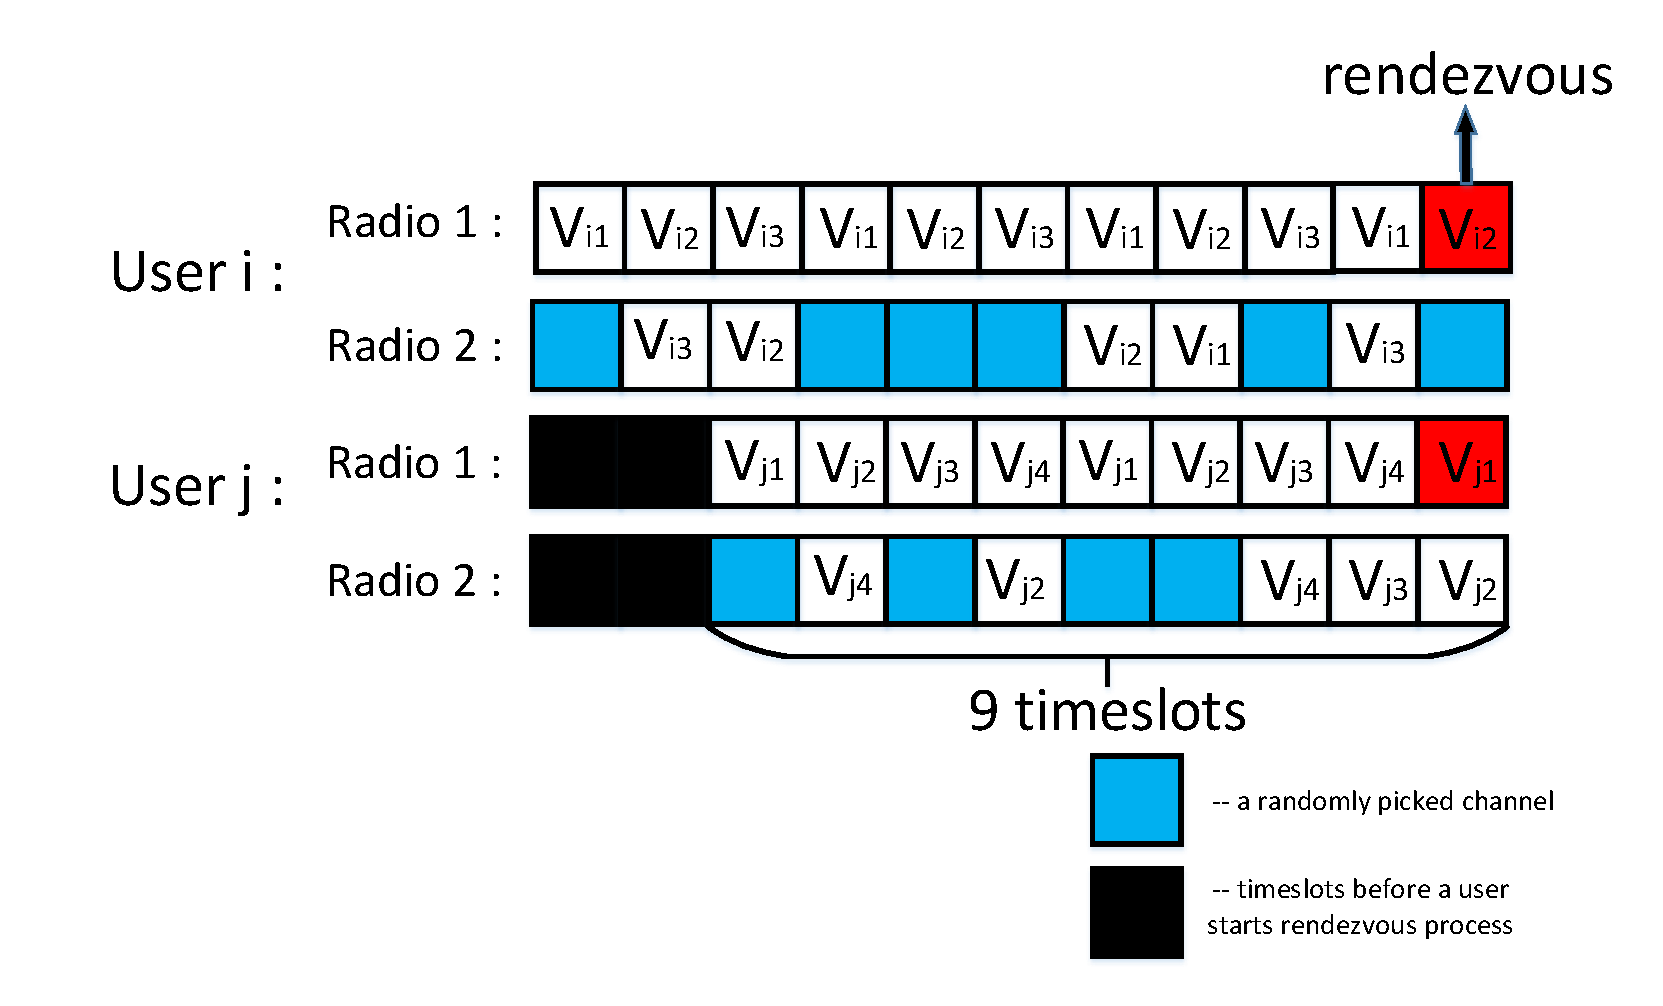
\includegraphics[width=1\columnwidth]{two-radio}
\caption{An example of Alg. {\ref{alg4}}.}
\label{two-radio}
\end{figure}



\begin{theorem}
Alg.\ref{alg4} can guarantee rendezvous for two users in $min\{|V_i|,|V_j|\}max\{P_i,P_j\}$ timeslots if $V_i \cap V_j \ne \emptyset$.
\end{theorem}

\begin{IEEEproof}
In Alg.\ref{alg4}, we use two radios to hop to channels according to different periods. The period of radio 1 is $m$ while the period of radio 2 is $P$. We then discuss in two cases:

\bfseries Case 1: \mdseries Suppose $m_i = m_j$. Let $m = m_i = m_j$. Then we divide this case into two subcases:

\bfseries Subcase 1.1: \mdseries Suppose $m$ is a prime. According to Alg.\ref{alg4}, $P_i = P_j = m + 1$ in this case. Let $P = m+1$. According to Lemma 2.3, $m$ and $P$ are co-prime. Hence, rendezvous can be achieved between $radio_{1i}$ and $radio_{2j}$ in $mP$ timeslots according to Theorem 2.

\bfseries Subcase 1.2: \mdseries Suppose $m$ is not a prime. Let $P =P_i=P_j$. $P$ is the smallest prime that $P > m$. According to Lemma 2.5, $m$ and $P$ are co-prime. Hence, rendezvous can be achieved between $radio_{1i}$ and $radio_{2j}$ in $mP$ timeslots according to Theorem 2.

\bfseries Case 2: \mdseries Suppose $m_i \ne m_j$.  Without lose of generality, suppose $m_i < m_j$. Then we divide this case into two subcases:

\bfseries Subcase 2.1: \mdseries Suppose $P_i = P_j = P$. In this case, $P$ must be a prime. Then according to Lemma 2.5, $m_i$ must be co-prime with $P$. Hence, rendezvous can be achieved between $radio_{1i}$ and $radio_{2j}$ in $mP$ timeslots according to Theorem 2.

\bfseries Subcase 2.2: \mdseries Suppose $P_i \ne P_j$. Then $P_i < P_j$. If $m_j$ is a prime, then according to Lemma 2.5, $m_j$ must be co-prime with $m_i$. Hence, rendezvous can be achieved between $radio_{1i}$ and $radio_{2i}$ in $m_im_j$ timeslots according to Theorem 2.
If $m_j$ is not a prime, $P_j$ must be a prime. $P_j$ must be co-prime with $m_i$. Hence, rendezvous can be achieved between $radio_{1i}$ and $radio_{2j}$ in $m_iP_j$ timeslots according to Theorem 2.

Combine these together, Theorem 4 holds.
\end{IEEEproof}

\begin{theorem}
The RD of Alg.\ref{alg4} is 100\%.
\end{theorem}

\begin{IEEEproof}
Both radio 1 and radio 2 of any user repeat a sequence periodically. For any two users i and j, there must exist one pair of co-prime numbers, one of which is in $m_i$ and $P_i$ and the other is in $m_j$ and $P_j$. In other words, one of the length of the period of $radio_{i1}$ and $radio_{i2}$ must be co-prime with that of $radio_{j1}$ or $radio_{j2}$. Denote the corresponding sequences as $S_i$ and $S_j$. From Theorem \ref{theo}, we know that every element in $S_i$ will meet all of the elements in $S_j$ and vice versa. Hence, the RD of Alg.\ref{alg3} is 100\%.
\end{IEEEproof}

\section{Semi-Synchronous Heterogeneous Rendezvous Algorithm}

In this section, we will propose a rendezvous for semi-synchronous model. In semi-synchronous model, we assume there exists a global clock, and the timeslots are aligned, but different users can start at different timeslots.

\begin{algorithm}
\caption{Semi-Synchronous Heterogeneous Rendezvous Algorithm}
\label{alg5}
\begin{algorithmic}[1]
\STATE Input: the set of available channels $V=\{v_1,v_2,\cdots,v_m\}$ and the total number of all channels: $N$ and the global time $T$;
\STATE Compute the number of timeslots passed from 00:00:00, denote it as $t$;
\WHILE{Not rendezvous}
\IF{Channel ($t\;\%N\;$ + 1) $\in V$}
\STATE Access Channel ($t\; \% \;N$ + 1);
\ELSE
\STATE Randomly pick a channel from $V$ and access it;
\ENDIF
\STATE $t:=t+1$;
\ENDWHILE
\end{algorithmic}
\end{algorithm}

The main idea of Alg.\ref{alg5} is very simple, which is to let users decide which channel to hop to based on the current global time. The line 2 of Alg.\ref{alg5} is to compute the timeslots passed from 00:00:00, which represents a baseline time. Here we suppose that the length of $N$ timeslots won't exceed a whole day. If we consider the time difference between time zones, this baseline time can be set to 00:00:00 of a fixed time zone.

\begin{theorem}
Alg.\ref{alg5} can guarantee rendezvous for two users in $N$ timeslots if $V_i \cap V_j \ne \emptyset$.
\end{theorem}

\begin{IEEEproof}
Without lose of generality, suppose user i begins not later than user j. Hence, when user j starts rendezvous process, user i is also in rendezvous process. In the following $N$ timeslots, user j will hop to all the available channels in $V$. If user i and user j has one common available channel, denote it as $c$, user i and j will hop to it simultaneously in one of the $N$ timeslots. Hence, rendezvous is achieved. Theorem 5 holds.
\end{IEEEproof}


\begin{figure}[!t]
\centering
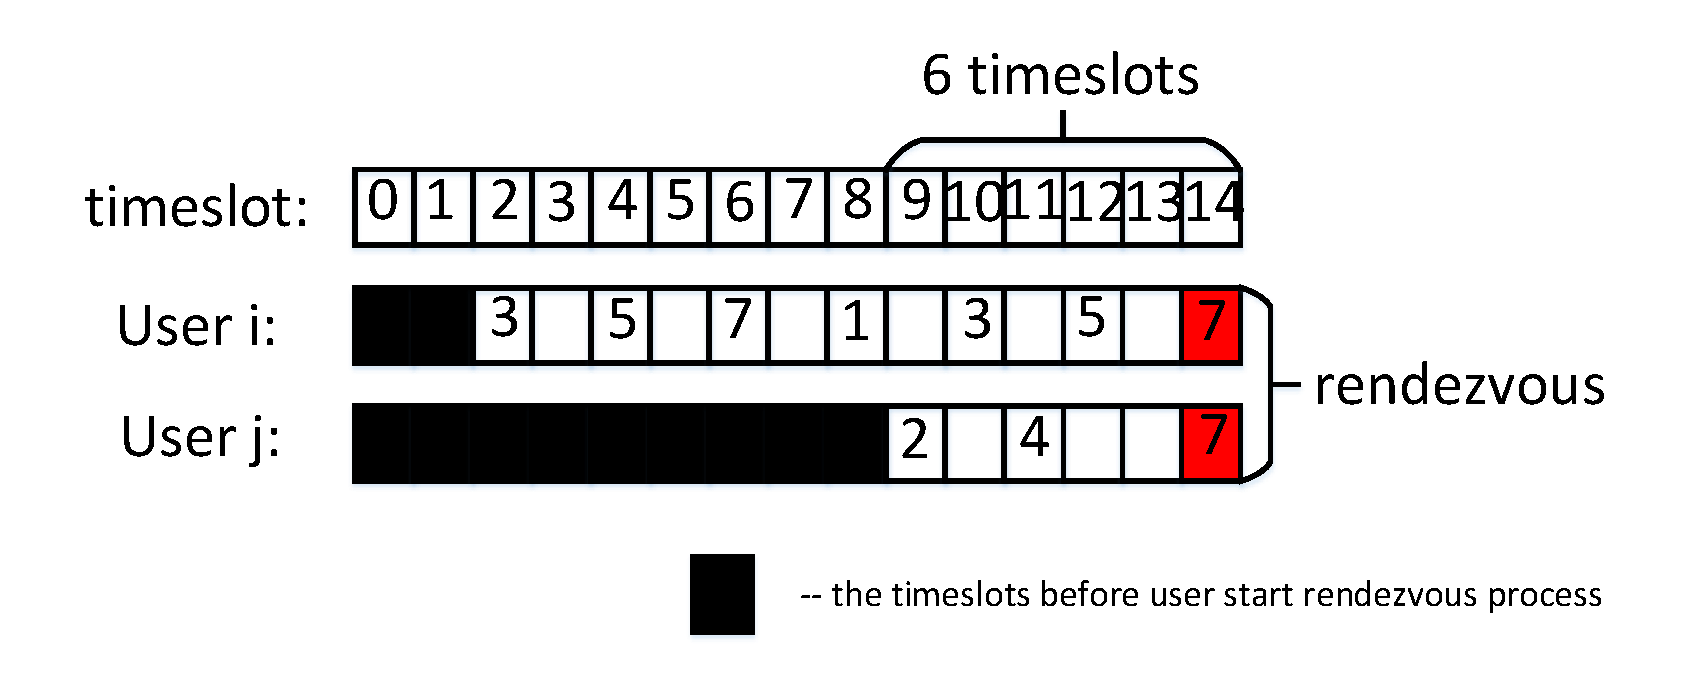
\includegraphics[width=1\columnwidth]{semi}
\caption{An example of Alg. {\ref{alg5}}.}
\label{exp_alg4}
\end{figure}

Fig.\ref{exp_alg4} illustrates an example of Alg.\ref{alg5}. In this example, $N$ is set to be 8. User i starts at the third timeslot and user j starts at tenth timeslot. $V_i = \{1,3,5,7\}$ and $V_j=\{2,4,7\}$. We can clearly see that TTR is $6 < 8$.

We need to point out that the timeslots don't need to be exactly aligned under the fundamental model. Because in fundamental model, the length of a timeslot is set to be 20 ms, from Fig.\ref{olp1} we know that as long as the accuracy of time is less than 10 ms. This is already achievable by using GPS or Beidou timing serive. Hence, semi-synchronous model is practical. And Alg.\ref{alg5} has the least MTTR compared with the existing rendezvous algorithms.

\begin{theorem}
The RD of Alg.\ref{alg5} is 100\%.
\end{theorem}

\begin{IEEEproof}
In Alg.\ref{alg5}, users will hop to all of their common channels in same timeslots. Hence, they will rendezvous at all of their common channels. Hence, the RD of Alg.\ref{alg5} is 100\%.
\end{IEEEproof}


\section{Simulation}

\section{Conclusion}

\section{Acknowledgements}



%\bibliographystyle{plain}
%\bibliography{references}
\end{document}


